\documentclass[conference]{IEEEtran}
\IEEEoverridecommandlockouts
% The preceding line is only needed to identify funding in the first footnote. If that is unneeded, please comment it out.
\usepackage{cite}
\usepackage{amsmath,amssymb,amsfonts}
\usepackage{algorithmic}
\usepackage{graphicx}
\usepackage{textcomp}
\usepackage{xcolor}
\usepackage{float}

% A todo macro for marking ToDos
\usepackage{color}
\newcommand{\todo}[1]{\textcolor{white}{\colorbox{blue}{ To do %
			:}}\textcolor{blue}{\ \ #1
	}\textcolor{blue}{\colorbox{blue}{III}}\ }
%\renewcommand{\todo}[1]{}

\def\BibTeX{{\rm B\kern-.05em{\sc i\kern-.025em b}\kern-.08em
    T\kern-.1667em\lower.7ex\hbox{E}\kern-.125emX}}
\begin{document}

\title{Projektdokumentation Smartstall\\
}

\author{\IEEEauthorblockN{1\textsuperscript{st} Hannes Bruhn}
\IEEEauthorblockA{\textit{Hochschule für angewandte Wissenschaften Coburg} \\
hannes\_bruhn@web.de}
\and
\IEEEauthorblockN{2\textsuperscript{nd} Florian Wermbter}
\IEEEauthorblockA{\textit{Hochschule für angewandte Wissenschaften Coburg} \\
florianwermbter@gmail.com}
}

\maketitle

\begin{abstract}
Hier steht das Abstract.
\end{abstract}

\begin{IEEEkeywords}
component, formatting, style, styling, insert
\end{IEEEkeywords}

\section{Hintergrund und Ziel des Projekts}
Das Projekt Smartstall ist im Rahmen des Moduls "Hardware cypher-physischer Systeme" des Master-Studiengangs Informatik entstanden, bei dem es um Schnittstellen und Datenübertragung von Endgeräten, sowie die Anbindung dieser an die Cloud nach dem Internet of Things (IoT) Konzept geht. \\
Ziel dieses Projekts ist die Erfassung unterschiedlicher Sensordaten zur Überwachung der Luftqualität in einem Stall. Die erfassten Daten sollen über einen Raspberry Pi an eine, für dieses Projekt entwickelte Webanwendung gesendet werden. Dadurch soll der Anwender die Möglichkeit erhalten, die Daten über eine benutzerfreundliche Oberfläche anzuzeigen und zu analysieren. Bei der Überschreitung von festlegbaren Schwellwerten bestimmter Attribute wie Temperatur, Luftfeuchtigkeit oder Ammoniakgehalt, soll der Anwender außerdem per Push-Up Benachrichtigung auf seinem Smartphone informiert werden können. \\
Des Weiteren soll die Belüftung von der Webanwendung bei Bedarf ein- und ausgeschaltet werden können, um die Schwellwerte auch ohne aktives Eingreifen des Anwenders wieder unterschreiten zu können. Dies soll durch die Ansteuerung einer WLAN-Steckdose umgesetzt werden. Durch regelmäßige und kontinuierliche Datenerfassung wird dafür gesorgt, dass die Belüftung nur so lange wie nötig aktiviert ist, womit die Aspekte Effizienz und Nachhaltigkeit berücksichtigt und in das Projekt integriert werden. 

\section{Hardware Komponenten}
\subsection{Raspberry Pi 3B}
Der Raspberry Pi (Modell 3B) ist ein beliebter Einplatinencomputer, der von der Raspberry Pi Foundation entwickelt wurde. Er bietet ausreichend Rechenleistung, Speicher und Konnektivität, um komplexe Aufgaben auszuführen und eine Vielzahl von Erweiterungen und Anwendungen zu unterstützen und ist somit ein kostengünstige und vielseitige Plattform für Projekte im Bereich der Einbettung von Computern und des IoT. Die umfangreiche Community und Dokumentation rund um den Raspberry Pi machen es einfach, Projekte zu starten und Unterstützung zu erhalten. Es gibt eine Vielzahl von Erweiterungsmodulen und Zubehörteilen, die den Raspberry Pi erweitern und an individuelle Anforderungen anpassen können. Um den Raspberry Pi 3B zu nutzen, ist eine grundlegende Einrichtung erforderlich, auf welche in Kapitel \ref{pi} genauer eingegangen wird. \cite{raspy} 

\subsection{Bosch Sensortec BME680 Sensor}
Der Bosch Sensortec BME680 ist ein fortschrittlicher Umweltsensor, der verschiedene Messungen in einer kompakten Einheit vereint. Der BME680 Sensor ermöglicht die Messung von vier Umweltparametern:
\begin{itemize}
	\item Temperatur: Der Sensor misst die Umgebungstemperatur mit hoher Präzision.
	\item Luftfeuchtigkeit: Er erfasst die relative Luftfeuchtigkeit und liefert genaue Feuchtigkeitswerte.
	\item Luftdruck: Der Sensor kann den atmosphärischen Druck messen und damit Wettervorhersagen ermöglichen.
	\item Luftqualität: Der BME680 Sensor ist in der Lage, flüchtige organische Verbindungen (VOCs) und verschiedene Gase wie Kohlenmonoxid (CO) und Stickstoffdioxid (NO2) zu erkennen.
\end{itemize}
Der BME680 Sensor findet Anwendung in einer Vielzahl von Bereichen, wie beispielsweise der Erfassung von Wetterdaten in Außenbereichen und der Überwachung von Luftqualität in Innenräumen. \cite{bme}
\subsection{MQ137 NH3-Gassensormodul}
Das MQ137 Gassensor-Modul ist ein Sensor, der speziell entwickelt wurde, um Ammoniakgas (NH3) in der Umgebungsluft zu messen. Er basiert auf der Metalloxid-Gassensortechnologie und erfasst die Konzentration von Ammoniak in Parts per Million (ppm). Der Sensor reagiert auf das Vorhandensein von Ammoniak, indem er Änderungen in der elektrischen Leitfähigkeit erkennt. Das MQ137 Gassensor-Modul ermöglicht eine präzise Erfassung von Ammoniakgas und findet Anwendung in verschiedenen Bereichen wie Industrie, Landwirtschaft und Umweltüberwachung.

\subsection{Verbinden der Komponenten}
Um die vorgestellten Sensoren nutzen zu können, müssen diese an die korrekten Pins des Raspberry Pis angeschlossen werden. Die zur Verfügung stehenden Pins des Raspberry Pis sind in Abbildung \ref{pi_pins} dargestellt.

\begin{figure}[H]
	\centering
	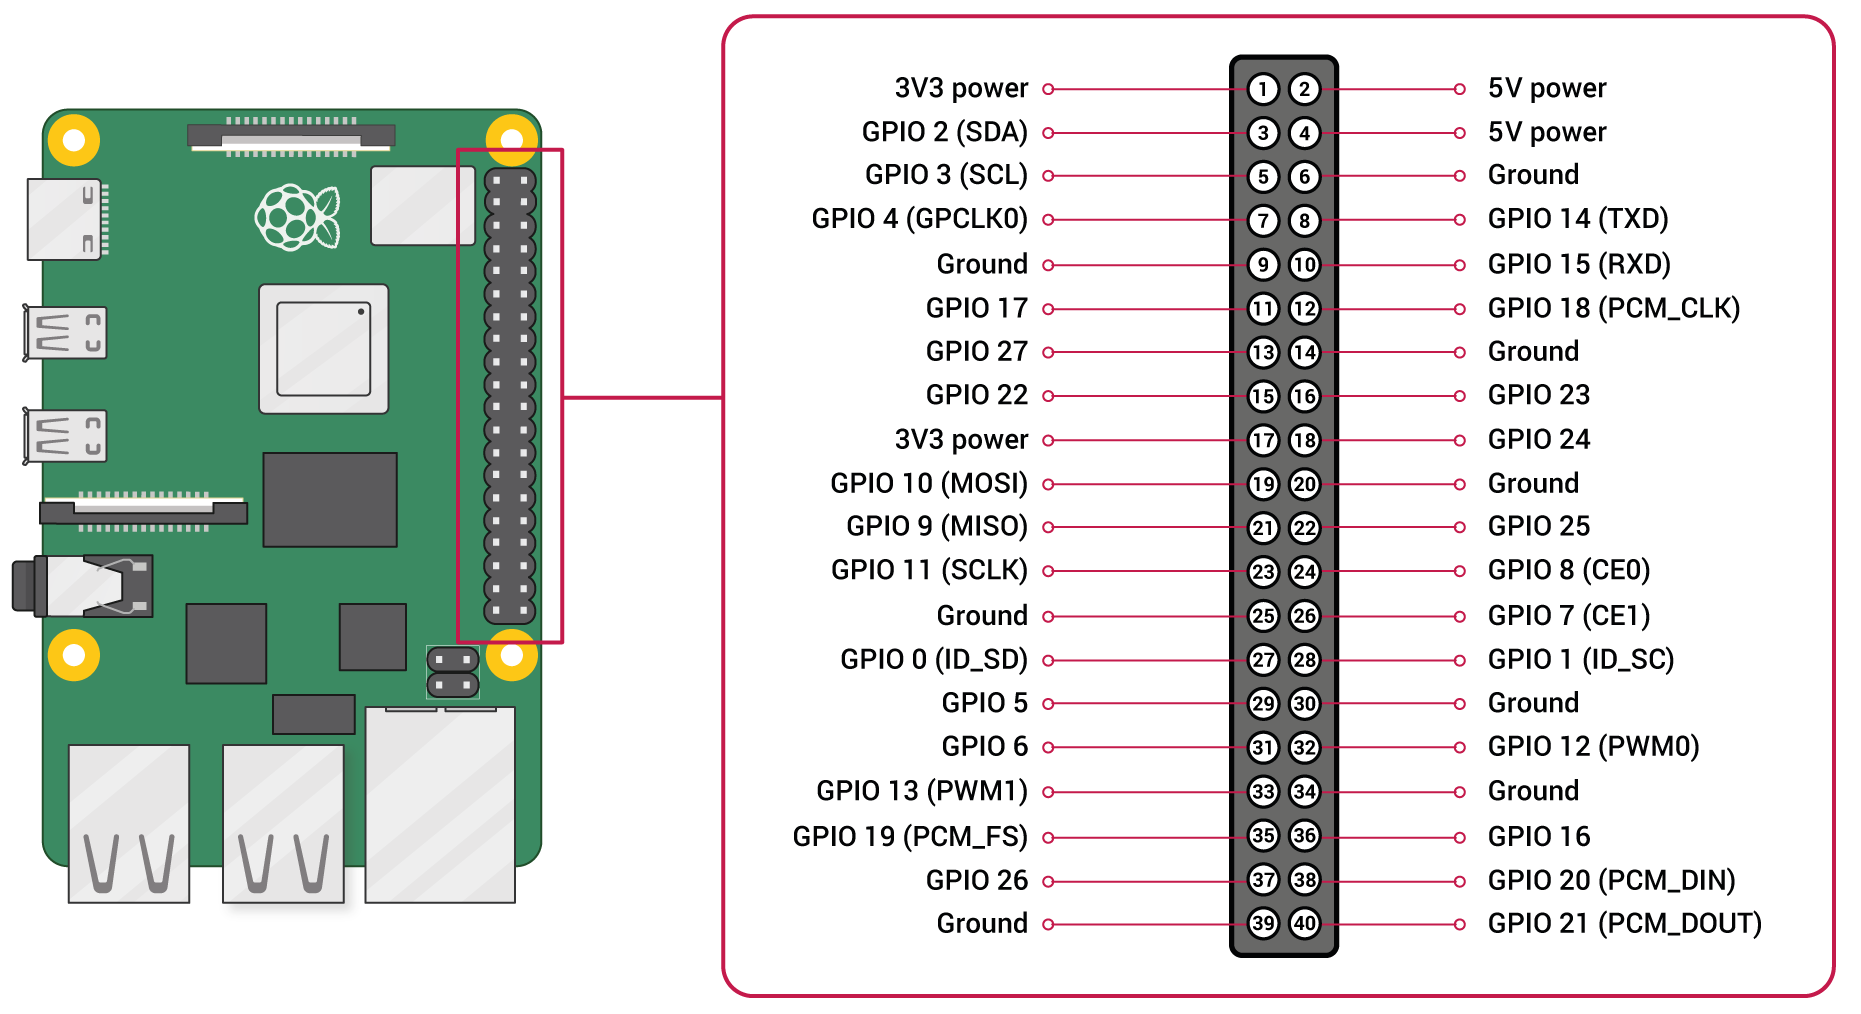
\includegraphics[width=90mm]{fig/pi_pins.png}
	\caption{Raspberry Pi 3B Pin Belegung}
	\label{pi_pins}
\end{figure}

\subsubsection{Anschließen des BME680 Sensors} 


Der BME680 besitzt sechs Pins, welche Abbildung \ref{bme_pins} zu entnehmen sind. Relevant sind hierbei die oberen 4 Pins, welche wie in Abbildung \ref{verkabelung_bme} aufgezeigt an den Raspberry Pi angeschlossen werden müssen. \cite{bme_anschluss}
\begin{figure}[H]
	\centering
	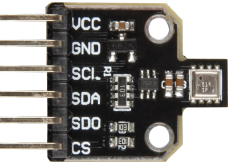
\includegraphics[width=50mm]{fig/bme_pins.png}
	\caption{BME680 Pins}
	\label{bme_pins}
\end{figure}
\begin{figure}[H]
	\centerline{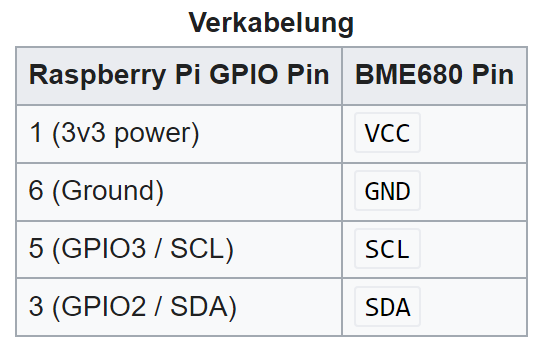
\includegraphics[width=50mm]{fig/verkabelung_bme.png}}
	\caption{Pin Verbindungen von Raspberry Pi und BME680}
	\label{verkabelung_bme}
\end{figure}

\subsubsection{Anschließen des MQ137 Sensors} 

Der MQ137 Sensor besitzt, wie in Abbildung \ref{mq137_pins} zu sehen 4 Pins, welche ebenfalls mit den jeweiligen Pins des Raspberry Pis verbunden werden müssen:
\begin{itemize}
	\item VCC: Stromversorgung (5V)
	\item GND: Ground
	\item DO: digitaler Signalausgang
	\item AO: analoger Signalausgang
\end{itemize}
\begin{figure}[H]
	\centerline{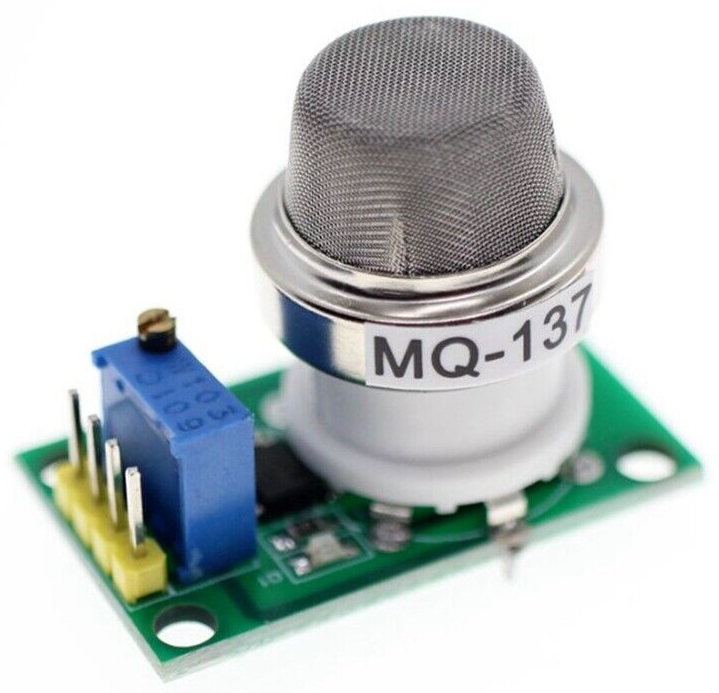
\includegraphics[height=40mm]{fig/mq137_pins.png}}
	\caption{MQ137 Gassensormodul}
	\label{mq137_pins}
\end{figure}

\subsubsection{Gesamtaufbau}
Die Sensoren wurden mittels Jumper-Kabeln und einem Breadboard mit dem Raspberry Pi verbunden. Der Aufbau und die beschriebene Verkabelung der Sensoren mit dem Raspberry Pi ist Abbildung \ref{aufbau} zu sehen.

\begin{figure}[htbp]
	\centerline{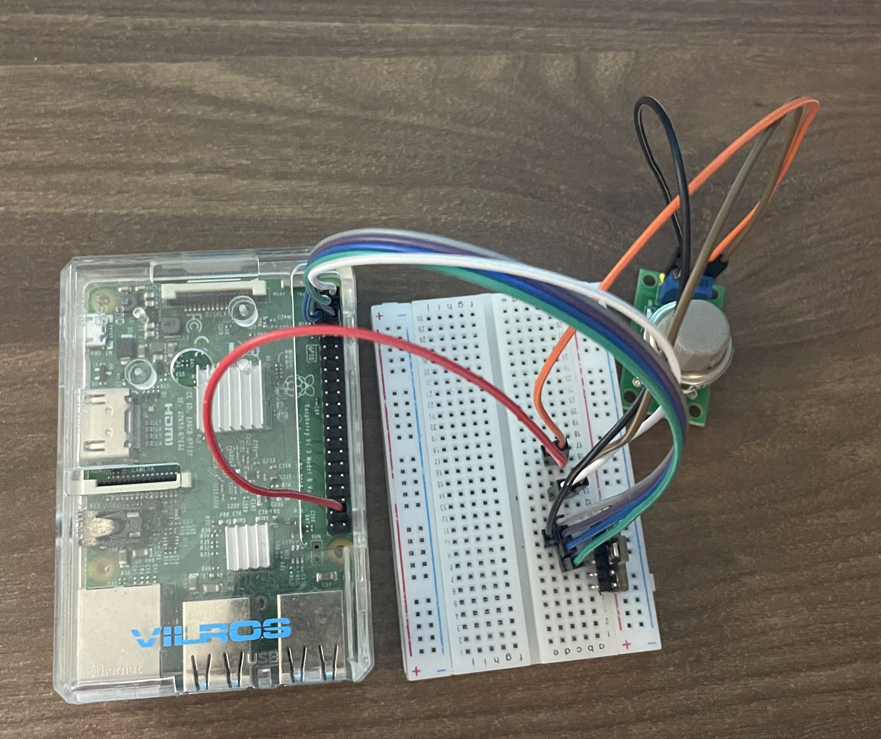
\includegraphics[width=80mm]{fig/aufbau.png}}
	\caption{Verkabelung der Sensoren mit dem Raspberry Pi}
	\label{aufbau}
\end{figure}

\section{Einrichtung Raspberry Pi}
\label{pi}
\subsection{Konfiguration}
Die erstmalige Einrichtung eines Raspberry Pi 3B umfasst mehrere Schritte, welche in diesem Kapitel aufgelistet werden. Zunächst eine Auflistung der benötigten und in diesem Projekt verwendeten Komponenten:
\begin{itemize}
	\item Raspberry Pi 3B
	\item MicroSD-Karte (mindestens 8 GB)
	\item Netzteil (5V)
	\item USB-Tastatur und -Maus
	\item HDMI-Kabel
	\item Bildschirm oder Fernseher mit HDMI-Eingang
\end{itemize}
Wenn das Anschließen von Ein- und Ausgabegeräten an den Raspberry Pi nicht gewünscht oder möglich ist, kann dieser nach der ersten Einrichtung alternativ auch über einen anderen Computer angesteuert werden, entweder per Remotedesktopverbindung oder per Kommandozeile mit Hilfe des Secure Shell (SSH) Netzwerkprotokolls. \cite{raspy} Zur erstmaligen Einrichtung muss zunächst das gewünschte Betriebssystem für den Raspberry Pi heruntergeladen werden, in diesem Fall Raspbian. Hierfür wurde das Program Raspberry Pi Imager von der offiziellen Raspberry Pi Website verwendet, welches die ausgewählte Version des Betriebssystems herunterlädt und diese direkt auf der MicroSD-Karte installiert. Anschließend kann die MicroSD-Karte in den Raspberry Pi eingesetzt und dieser gestartet werden. Für die Einrichtung muss nun lediglich den Anweisungen auf dem Bildschirm gefolgt werden, anschließend kann der Raspberry Pi über die grafische Benutzeroberfläche verwendet oder über Konsole angesteuert werden.  


\subsection{Software und Bibliotheken}
Nach der Einrichtung des Raspberry Pi musste zunächst das I2C (Inter-Integrated Circuit) Interface über die raspi-config aktiviert werden. I2C  ist ein serieller Kommunikationsbus zur Verbindung von elektronischen Bauteilen über nur zwei Datenleitungen: SDA (Serial Data Line) und SCL (Serial Clock Line). Es ermöglicht die einfache Kommunikation zwischen verschiedenen Geräten wie Mikrocontrollern, Sensoren und Aktoren. Dieser wird vom BME680 Sensor zur Übertragung der Messwerte genutzt. Da für das Abfragen der Sensordaten in diesem Projekt Python verwendet wird, welches bereits standardmäßig mit dem Raspian Betriebssystem mitinstalliert wird, müssen zusätzlich noch einige Bibliotheken installiert werden: 
\begin{itemize}
	\item python3-smbus: Ermöglicht die Kommunikation über in I2C-Bus in Python. Es werden Funktionen bereitgestellt I2C-Geräte anzusprechen und Daten zu senden und zu empfangen.
	\item i2c-tools: Wird für die Verwaltung und Diagnose des I2C-Busses verwendet. Dies bietet zusätzliche Funktionalitäten wie das Anzeigen angeschlossener Geräte.
	\item adafruit-circuitpython-bme680: 
\end{itemize}

\subsection{Datenübertragung}


\section{Webanwendung}
\subsection{Architektur und Design}
\subsection{Empfangen der Daten}
\subsection{Anbindung einer MYSQL Datenbank}
\subsection{Auslesen und Anzeigen der Sensordaten}
\subsection{Benutzeroberfläche}
\subsection{Telegram Anbindung}
\subsection{Ansteuerung der Steckdose}


\begin{thebibliography}{00}
\bibitem{raspy}
Raspberry Pi Foundation, "Raspberry Pi", Online. Verfügbar unter: https://www.raspberrypi.com. [Zugriffsdatum: 10. Juli 2023].
\bibitem{bme}
Joy-It, "BME680", Online. Verfügbar unter: https://joy-it.net/de/products/SEN-BME680. [Zugriffsdatum: 10. Juli 2023].
\bibitem{bme_anschluss}
Laub-Home Wiki, "Raspberry Pi BME680 Gas Sensor", Online. Verfügbar unter: https://www.laub-home.de/wiki/Raspberry\_Pi\_BME680\_Gas\_Sensor. [Zugriffsdatum: 12. Juli 2023].
\end{thebibliography}

\end{document}
